\documentclass[twocolumn,10pt]{article}
\usepackage{authblk}
\usepackage{bera}
\usepackage[utf8]{inputenc}
\usepackage[T1]{fontenc}
\usepackage{graphicx}
\usepackage{booktabs}
\usepackage{float}
\usepackage{url}
\usepackage{microtype}
\usepackage[margin=1in]{geometry}
\setlength{\textfloatsep}{8pt plus 2pt minus 2pt}
\setlength{\floatsep}{8pt plus 2pt minus 2pt}
\setlength{\dbltextfloatsep}{8pt plus 2pt minus 2pt}
\graphicspath{{figures/}}
\title{Specialty Classification of Clinical Notes:\\Representations, Metadata and Repeated Notes}
% Replace with the actual group number, names and contribution percentages.
\author{Group 14\\
Antero Morgado (119213; XX\%), António Palma (119203; XX\%)\\
Martim Godinho (106565; XX\%), Tomás Tenrinho (121374; XX\%)}
\date{}
\begin{document}
\maketitle

\section{Introduction}
We classify clinical notes into 12 specialties using their description, sample name, transcription and keywords. Data inspection revealed that the first keyword often names the specialty, while identical notes can have different labels. Our research question is: \textbf{How do lexical and pretrained representations compare when specialty metadata is available versus absent, and when notes are repeated versus unseen?} We separate model predictions from explicit keyword and duplicate rules to measure these effects. 

\section{Data}
\subsection{Data Analysis}
Of 2,616 records, three contain note fragments instead of valid labels and have empty clinical fields; excluding them leaves 2,613. Surgery has 876 cases and Dermatology 25 (35:1); 441 cases lack keywords and 30 lack transcriptions. Table~\ref{tab:classes} gives the class distribution.

\textbf{Specialty keywords.} Of 2,172 keyword lists beginning with a specialty name, 2,171 match the label. Thus metadata can dominate predictions.
\textbf{Conflicting copies.} There are 712 repeated cleaned-note groups, 711 with conflicting labels; in 710, every copy has a different specialty. For example, ``Left lower extremity venous Doppler ultrasound'' occurs under both Cardiovascular-Pulmonary and Radiology.
\textbf{Formatting faults.} Seven descriptions contain embedded records. Shared cleaning truncates them at the first embedded record and normalises the \texttt{.,} section separators, identically at fitting and inference.

\subsection{Data Augmentation}
We target the four smallest classes (Dermatology, Psychiatry-Psychology, Ophthalmology and Neurosurgery), towards 150 cases each, with at most four variants per original. We compare \emph{resampling} (copies), \emph{field dropout} (remove keywords; remove sample name with probability 0.5 and transcription with probability 0.35 when a description remains), and \emph{section recombination}. The latter replaces each headed section, with probability 0.5, with a same-header section from another fitting-fold note of the same class. All originals and donors remain inside the fitting fold. Resampling controls for minority-example frequency.

\section{Models}
We compare six representation families, informed by the course \cite{coheur2026}.
\textbf{Naive Bayes (NB)} uses lowercased, Porter-stemmed description TF-IDF with multinomial NB ($\alpha=1$), matching the specified weak baseline.
\textbf{Word logistic regression (LR)} uses TF-IDF from all available fields.
\textbf{Word/character SVM} combines field-specific word and character features.
\textbf{Latent semantic analysis (LSA) + LR} compresses word TF-IDF into 128 dimensions.
\textbf{Frozen MiniLM + LR} uses \texttt{all-MiniLM-L6-v2} \cite{reimers2019,wang2020,minilmcard}; averaging 220-token chunks yields a 384-dimensional vector per field, concatenated into 1,536 dimensions.
\textbf{ClinicalBERT} fully fine-tunes \texttt{Bio\_ClinicalBERT} \cite{alsentzer2019}. Since 70.8\% of notes exceed 512 tokens, we compare the first 510 word pieces with the first 128 plus last 382, reserving two special tokens. A classifier reads the 768-dimensional [CLS] representation.

Inputs either omit keywords, remove only the first keyword, or retain all keywords. A \textbf{keyword rule} takes priority: map the first keyword using fixed specialty names or fitting-data mappings with at least two observations and 95\% purity. A \textbf{duplicate rule} excludes labels already attached to an identical fitting note and selects the highest remaining model score. This exploits a corpus regularity, rather than a clinical principle.

\section{Experimental Setup}
We compare stratified \emph{random} partitions, allowing repeated notes across boundaries, with \emph{grouped} partitions, keeping cleaned transcription copies together (other clinical fields identify empty-transcription cases). Seeded five-fold splits yield 1,672 fitting, 418 validation and 523 held-out cases. We evaluate only the first outer/inner folds. Models fit identical rows; selection prioritises validation macro-F1, minimum class F1, then accuracy.

Choices are frozen after validation. The winner is refitted on all 2,613 labelled cases to predict the 398 unlabelled official inputs, used only for \texttt{results.txt}. We report accuracy, macro/per-class F1 and note-group bootstrap intervals.

\subsection{Parameters/Hyperparameters}
Partition and neural seeds are 20261008 and 42. We search inverse regularisation strength $C\in\{0.3,1,3\}$ for SVM and $\{1,10\}$ for LR, with ordinary or balanced class weights. Larger $C$ weakens regularisation. SVM uses word 1--2-grams (minimum document frequency 2, cap 40,000 per field) and character 3--5-grams within word boundaries (minimum 3, cap 30,000). Word LR/LSA use word 1--2-grams (minimum 2, cap 60,000). TF is sublinear and vectors are L2-normalised. ClinicalBERT uses AdamW, learning rate $3\times10^{-5}$, weight decay 0.01, 10\% warm-up, square-root inverse-frequency class weights, three epochs and effective batch 16 (micro-batches of eight, gradient accumulation two). MiniLM/ClinicalBERT revisions are pinned in the code and references. Runs used an Apple M4 with 16\,GB; software includes scikit-learn \cite{pedregosa2011}, PyTorch, Transformers and Sentence Transformers.

\section{Results}
Table~\ref{tab:models} compares validation-selected bare models, with the first specialty keyword removed (NB uses description only). The submitted system is an \textbf{unaugmented SVM}, $C=0.3$, balanced weights, no keyword input, plus both rules. It achieves \textbf{95.79\% accuracy, 0.9402 macro-F1 and 0.8000 minimum class F1} on the random held-out set; the 95\% macro-F1 interval is [0.897, 0.969]. The separately selected grouped system achieves 93.50\% accuracy and 0.9141 macro-F1. These are internal results, not official-test scores. Table~\ref{tab:classes} gives per-class performance; Figure~\ref{fig:confusion} shows the full confusion matrix.

\begin{table}[!ht]
\centering\small
\setlength{\tabcolsep}{3pt}
\begin{tabular}{lrrrr}
\toprule
& \multicolumn{2}{c}{Random} & \multicolumn{2}{c}{Grouped}\\
Model & Acc.\% & F1 & Acc.\% & F1\\\midrule
NB &36.5&.099&40.7&.143\\
Word LR &46.7&.502&57.2&.594\\
Word/char SVM &41.1&.419&59.3&.615\\
LSA + LR &51.8&.542&54.7&.565\\
MiniLM + LR &50.1&.542&58.5&.620\\
ClinicalBERT &53.9&.537&57.2&.604\\\bottomrule
\end{tabular}
\caption{Bare models on common held-out partitions; F1 is macro-averaged.}\label{tab:models}
\end{table}

\begin{table}[!ht]
\centering\small\setlength{\tabcolsep}{3pt}
\begin{tabular}{lrrrrr}
\toprule
Specialty & $N$ & $n$ & P & R & F1\\\midrule
Cardio-Pulmonary &299&60&.95&.98&.97\\
Dermatology &25&5&.80&.80&.80\\
Gastroenterology &192&39&1.00&.90&.95\\
General Medicine &207&41&.81&.95&.88\\
Neurology &181&36&.97&.92&.94\\
Neurosurgery &78&16&.89&1.00&.94\\
Obstetrics-Gynecology &135&27&1.00&.93&.96\\
Ophthalmology &71&14&1.00&1.00&1.00\\
Orthopedic &292&58&.96&.95&.96\\
Psychiatry-Psychology &40&8&1.00&.88&.93\\
Radiology &217&44&.96&1.00&.98\\
Surgery &876&175&.99&.97&.98\\\bottomrule
\end{tabular}
\caption{Submitted system on the random held-out set. $N$: full labelled-corpus count; $n$: held-out support; P/R: precision/recall.}\label{tab:classes}
\end{table}

\begin{figure}[H]
\centering
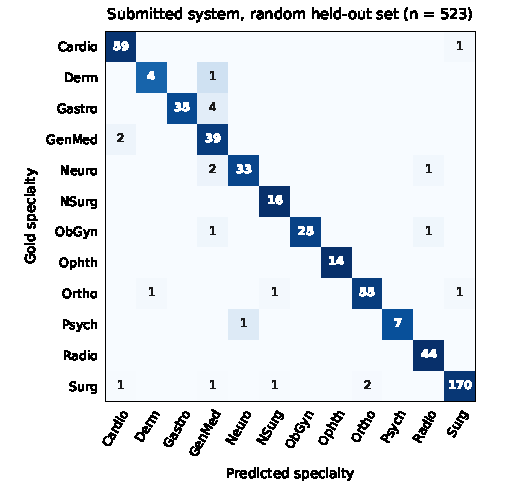
\includegraphics[width=\columnwidth]{fig1_submitted_random.pdf}
\caption{Full confusion matrix of the submitted system on 523 random held-out cases: rows are gold labels, columns predictions; counts are shown, with colour normalised by row. Specialty abbreviations follow Table~\ref{tab:classes} in the same order.}\label{fig:confusion}
\end{figure}

\section{Discussion}
\textbf{Representations and repeated notes.} Grouped macro-F1 ranges from 0.565 to 0.620 for non-baseline bare models, with no clear large pretraining advantage in this single-fold comparison. Of 190 repeated random held-out notes, 189 have a gold label different from their fitting copy's. The bare SVM always repeats a previously seen label: 0\% accuracy on repeated cases versus 64.6\% on unseen cases. Conflicting labels therefore make memorisation harmful.

\textbf{Metadata and rules.} The keyword rule decides 444/523 cases, all correctly; duplicate exclusion decides 25 (76.0\% correct), leaving 54 to the SVM (70.4\%). Fixed SVM ablations raise random macro-F1 from 0.399 without keywords to 0.885 with all keywords, or 0.945 with both rules (a different configuration from the submission). These gains reflect corpus structure, not demonstrated performance on untagged notes.

\textbf{Augmentation.} Table~\ref{tab:aug} shows only small gains: resampling adds 0.004--0.008 macro-F1, recombination 0.003--0.006; dropout reduces it by 0.011--0.016. Recombination does not outperform simple copies. It can also join incompatible content: an eyelid-repair title from note 1110 accompanies lens-removal text from note 1143. The validation-selected submission uses no augmentation.

\textbf{Errors.} The submitted system makes 22 mistakes; the most common pair is Gastroenterology predicted as General Medicine (four). Three concrete examples illustrate different failure modes:

\textbf{Note 361:} ``I was asked to see the patient for C. diff colitis.'' Predicted \emph{General Medicine}; gold \emph{Gastroenterology}. With no keywords, the long admission history may obscure the gastrointestinal cue.

\textbf{Note 2582:} ``Primary right shoulder arthroscopic rotator cuff repair with subacromial decompression.'' Predicted \emph{Orthopedic}; gold \emph{Surgery}. The procedure fits both specialties, illustrating ambiguity in a single-label target.

\textbf{Note 771:} ``Left third digit numbness and wrist pain.'' Predicted \emph{Radiology}; gold \emph{Neurology}. A fitting copy is labelled Orthopedic, which duplicate exclusion removes. The remaining prediction is consistent with the sample name ``MRI C3 - Cord Compression''; exclusion alone cannot identify the correct alternative.

Small class supports, one fold, retrospective exploration and corpus-specific rules limit generalisation; exact matching misses near-copies. The errors suggest label overlap, without proving labels incorrect. Lexical and pretrained models perform similarly on unseen notes; metadata and conflicting repetition dominate full-system results.

\section{Future Work}
Repeat outer folds and seeds; test clinically coherent augmentation, whole-note encoding and multi-label targets for overlapping specialties. Evaluate a lexical/neural ensemble only if validation supports it.

\paragraph{Declaration of LLM use.}
Claude (Anthropic) and OpenAI helped synthesise course material, implement code, perform complex technical tasks and prepare the report. The group used this support to inform its approach, made all design and methodological choices, and remains responsible for the implementation, analysis and conclusions.

% The main paper ends here; bibliography is excluded from its three-page limit.
\clearpage
\ifnum\value{page}>4 \errmessage{Main paper exceeds three pages}\fi
\bibliographystyle{apalike}
\bibliography{biblio}

\clearpage
\onecolumn
\newcounter{appendixstart}
\setcounter{appendixstart}{\value{page}}
\appendix
\section*{Appendix A: Extra Figures and Tables}

\begin{table}[H]
\centering\small
\begin{tabular}{llrrr}
\toprule
Regime & Augmentation & Accuracy (\%) & Macro-F1 & Minority mean F1\\\midrule
Random & None &43.2&.441&.440\\
& Resampling &43.2&.445&.451\\
& Field dropout &43.2&.430&.405\\
& Section recombination &43.0&.444&.450\\
Grouped & None &59.3&.608&.618\\
& Resampling &59.5&.616&.638\\
& Field dropout &58.9&.592&.566\\
& Section recombination &59.4&.614&.633\\\bottomrule
\end{tabular}
\caption{Augmentation diagnostics: three-fold pooled predictions within the outer development partition, distinct from the held-out results in Table~\ref{tab:models}. Minority mean F1 averages the four augmented classes.}\label{tab:aug}
\end{table}
\clearpage
\addtocounter{appendixstart}{1}
\ifnum\value{page}>\value{appendixstart} \errmessage{Appendix exceeds one page}\fi
\end{document}
